\documentclass[a4paper]{article}

%% Language and font encodings
\usepackage[brazil,english]{babel}
\usepackage[utf8]{inputenc}
\usepackage{indentfirst}
%% Sets page size and margins
\usepackage[a4paper,top=3cm,bottom=2cm,left=3cm,right=3cm,marginparwidth=1.75cm]{geometry}

%% Useful packages
\usepackage{amsmath}
\usepackage{graphicx}
\usepackage[colorinlistoftodos]{todonotes}
\usepackage[colorlinks=true, allcolors=blue]{hyperref}
\usepackage{listings}
\usepackage{color}
\lstset{ %
  language=R,                     % the language of the code
  basicstyle=\footnotesize,       % the size of the fonts that are used for the code
  numbers=left,                   % where to put the line-numbers
  numberstyle=\tiny\color{gray},  % the style that is used for the line-numbers
  stepnumber=1,                   % the step between two line-numbers. If it's 1, each line
                                  % will be numbered
  numbersep=5pt,                  % how far the line-numbers are from the code
  backgroundcolor=\color{white},  % choose the background color. You must add \usepackage{color}
  showspaces=false,               % show spaces adding particular underscores
  showstringspaces=false,         % underline spaces within strings
  showtabs=false,                 % show tabs within strings adding particular underscores
  frame=single,                   % adds a frame around the code
  rulecolor=\color{black},        % if not set, the frame-color may be changed on line-breaks within not-black text (e.g. commens (green here))
  tabsize=2,                      % sets default tabsize to 2 spaces
  captionpos=b,                   % sets the caption-position to bottom
  breaklines=true,                % sets automatic line breaking
  breakatwhitespace=false,        % sets if automatic breaks should only happen at whitespace
  title=\lstname,                 % show the filename of files included with \lstinputlisting;
                                  % also try caption instead of title
  keywordstyle=\color{blue},      % keyword style
  commentstyle=\color{teal},   % comment style
  stringstyle=\color[rgb]{1,0,0},      % string literal style
  escapeinside={\%*}{*)},         % if you want to add a comment within your code
  morekeywords={*,...}            % if you want to add more keywords to the set
}

\addto\captionsenglish{\renewcommand{\figurename}{Figura}}
\renewcommand{\lstlistingname}{Código}
\renewcommand{\t}{Código}
\usepackage{caption}
\captionsetup[table]{name=Tabela}

\title{Estatísticas para um Melhor Desempenho no League of Legends}
\author{Iverson Pereira e Ricardo Luna}

\begin{document}
\maketitle

\begin{abstract}
Jogos Online etão cada vez mais populares nas últimas décadas. Um desses jogos é \textit{League of Legends}. Este jogo possui milhões de jogadores diários o que gera uma massa de dados enorme a cada segundo. Diante disso, este projeto visa propor estatísticas para auxiliar jogadores durante suas partidas no jogo. Utilizamos funções da linguagem R com auxilio de outros pacotes para trabalhar em cima de uma base de dados com mais de 12 mil partidas. Apresentamos gráficos para ajudar o jogador a definir possíveis personagens levando em consideração os desafios da versão atual do jogo. Além disso, prevemos resultados de partidas utilizando o algoritmo kNN.
\end{abstract}

\section{Introdução}

\textit{League of Legends}\footnote{https://br.leagueoflegends.com/} (popularmente conhecido como LoL) é um jogo disponível online estilo MOBA (\textit{Multiplayer Online Bale Arena}) e também possui fortes elementos de RPG (\textit{Role-Playing Game}). Dentre outras características o jogo tem apresentado dados bastantes significativos nos últimos anos. Em 2017, o cenário competitivo teve um faturamento de U\$12,016,606.24 como um total de 135 campeonatos nesse período o que representa um dos maiores faturamentos em jogos desse estilo.  

O jogo teve sua inspiração em outro jogo chamado Dota\footnote{http://br.dota2.com/} (\textit{Defense of the Ancients}). Dota tem como objetivo a destruição de uma estrutura principal para condição de vitória da partida. Essa estrutura de jogo também é comum ao LoL com adição de outros elementos próprios: rota de selva, dragões elementais e outros recursos que fornecem maiores vantagens para equipe.  

O jogo tem apresentado aspectos bastantes interessantes mais recentemente, a cada nova sessão, atualização grande que traz mudanças maiores ao jogo, ou a cada novo \textit{patch} que são atualizações menores visando o balanceamento e resolver problemas no jogo. Isso possibilita que jogadores mais experientes descubram ou proponham novas formas de jogo e composições objetivando um melhor desempenho e consequentemente aumentando suas chances de vitória. 


Assim como mostrado na Figura~\ref{fig:map}, o jogo possui quatro rotas: \textit{top} (superior), \textit{mid} (meio), bot (inferior) e \textit{jungle} (selva). Cada uma dessas rotas possui uma característica própria e com isso o os personagens que jogam nessas rotas devem cumprir certos requisitos.  No topo é utilizando normalmente um personagem capaz que ficar vivo durante um longo tempo nas lutas e sofre boa parte do dano que seria direcionado aos jogadores de seu time. Já na rota do meio, geralmente são utilizados personagens com um dano por segundo (\textit{dps}) alto e assim eliminar os jogadores do time inimigo que possam causar mais dano ao seu time. Os jogadores da rota inferior, que são geralmente dois, são o ADC (\textit{Attack Damage Carry}), que tem como função causar grandes cargas de dano ao time inimigo e geralmente esses personagens possuem ataque a longa distância, e o suporte é o responsável por manter o ADC vivo, geralmente deve possuir habilidades para auxiliar os outros jogadores como curas, escudos e controles de grupo visando causar algum atraso ou retardar o ataque da equipe inimiga. 

\begin{figure}[ht]
\centering
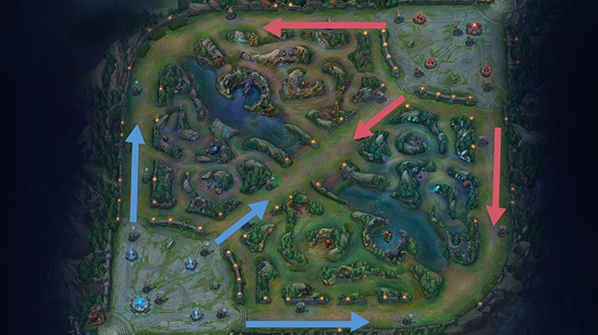
\includegraphics[width=0.7\textwidth]{imagens/rotas}
\caption{\label{fig:map}Mapa do Summoner's Rift. \cite{leol}}
\end{figure}

Mas como já mencionado o jogo vem trazendo mudanças mais frequentes e isso tem ``forçado" uma adaptação mais rápida de seus jogadores. O META, como essa adaptação é chamada, pode ser visto como um estilo que ao longo do tempo vem se mostrando mais efetivo que os outros e aproveita mais efetivamente os recursos disponíveis. Mas a pergunta que fica é ``como se adaptar de forma mais rápida ao META?".  Diante deste questionamento, este trabalho tenta trazer uma resposta. De forma simples o trabalho mostra uma análise baseada em estatísticas do jogo visando mostrar quais os personagens estão mais fortes, no \textit{patch} atual, ou quais personagens melhor se adaptam ao novo META.  

O projeto deve utilizar uma base de dados retirada do site OP.GG\footnote{http://br.op.gg/}. Esta base de dados possui um histórico de todas as partidas realizadas no jogo e outras informações relacionadas. Com um total de mais de 12 mil partidas, os dados representam informações cruciais do jogo. Listamos abaixo estas informações: 

\begin{itemize}
	\item Personagens utilizados em cada equipe;
    
	\item Resultado final da partida, derrota ou vitória;
    
    \item Liga, que indica qual o ``nível" ou ranking dos jogadores;
    
    \item \textit{Patch} no qual o jogo foi realizado;
    
    \item Região onde ocorreu o jogo.
\end{itemize}  


O trabalho deve oferecer um conjunto de estatísticas que serão descobertas a partir dos dados. Dentre elas, propomos estatística para taxa de vitória por personagem, popularidade de cada personagem por região (baseado na quantidade de partidas jogadas) e também o uso do k-NN (\textit{k-Nearest Neighbors}). O uso do k-NN tem a finalidade de prever o time vencedor utilizando dois times como entrada para o algoritmo. Esta previsão é baseada na análise do conjunto de dados estatísticos gerado, para que se possa afirmar quais composições terão maiores chances de ganhar ou não uma partida. Diante disso, o jogador pode utilizar essas informações baseadas em estatística para auxiliá-lo e, dessa forma, obter um maior conhecimento sobre o jogo de forma rápida e confiável.

\section{Pacotes Requeridos}

Para executar essa análise é preciso instalar e carregar alguns pacotes específicos que não são nativos em R. Os pacotes utilizados para essa análise de dados estão dispostos no Código~\ref{cod:library}. O pacote \texttt{tidyr} é utilizado para ajustar tabelas, como por exemplo, transformar colunas em linhas com o comando \texttt{gather}. O pacote \texttt{dplyr} é usado para manipulação dos dados para facilitar a obtenção de informações com o uso de funções como \texttt{group\_by} e \texttt{summarise}. A biblioteca \texttt{stringr} é importada para auxiliar em operações com \textit{strings}.

\begin{lstlisting}[language=R, caption={Pacotes utilizados no projeto},label={cod:library}]
#Carrega os pacotes necessarios
library(tidyr) #Ajustar os dados
library(dplyr) #Manipular os dados
library(stringr) #Operacoes com string
\end{lstlisting}

\section{Preparação dos Dados}
Esta seção apresenta os dados na sua forma original e descreve as etapas executadas para realizar a limpeza dessa massa de dados, a fim de possibilitar a extração de estatísticas posteriormente. A Seção~\ref{sec:fontedados} explica como os dados foram obtidos. Na Seção~\ref{sec:entendendo} os dados são expostos e explicados. Finalmente, na Seção~\ref{sec:limpeza} é mostrado como é realizada a limpeza e formação dos dados a partir do conjunto de dados original.

\subsection{Fontes dos dados}
\label{sec:fontedados}
Para a obtenção da base de dados utilizamos um projeto do GitHub chamado LOL.tools\footnote{em https://github.com/MarcusDEFGH/LOL.tools}. Este projeto utiliza o Scrapy\footnote{https://scrapy.org/}, biblioteca em Python, que coleta os dados de uma página web e gera um arquivo .\texttt{csv} com os dados capturados. O site de onde os dados são extraídos é o OP.GG. Como já mencionado esse site disponibiliza um histórico de todas as partidas do jogo e tal dado é divido por regiões, onde cada região representa os servidores implantados. O arquivo gerado está disponível pelo link https://raw.githubusercontent.com/RicardoLuna/LOL\_STATISTICS/master/patch811.csv.

\subsection{Entendendo os Dados}
\label{sec:entendendo}
Os dados coletados são relacionados as ligas do disponíveis no jogo (bronze, prata, ouro, platina, diamante, mestre e desafiante), cada liga representa um nível de habilidade do jogador. Para ser classificado em uma liga, o jogador deve jogar 10 partidas e a partir do seu desempenho o jogador será classificado. Todos as ligas começam no nível 5 e vão no máximo até o 1. Para subir entre os níveis, de uma mesma liga, o jogador deve jogar 3 partidas, quando atingir o limite de 100 Pontos de Liga (PdL), se obtiver duas vitórias o jogador é promovido. Para conseguir subir de liga o jogador deve chegar no nível 1 da liga e obter 100 PdL e caso consiga vencer 3 das 5 partidas que devem ser disputadas o jogador é promovido. Quando se chega no ouro o jogador ganha um conjunto de itens dentro do jogo a cada sessão, geralmente no início do ano, e ao se chegar no desafiante o jogo envia presentes para os jogadores de cada região. Geralmente nas equipes competitivas os jogadores escolhidos são do nível desafiante e a premiação é maior nos campeonatos. 

Os dados correspondem a partidas realizadas no período de 31 de Maio à 18 de Junho de 2018. Estes dados, retirados a partir da fonte mencionada na seção anterior, são compostos por um total de 14 colunas; as linhas representam as partidas, na Figura~\ref{fig:dataantes} está ilustrado parte dessa massa de dados. As 10 primeiras colunas representam os integrantes (personagens) dos times. Os personagens do primeiro time são representados pelos valores das colunas $team_1.x$, onde \textit{x} varia de 0 até 4.  Os personagens do time 2 são representados pelas colunas $team_2.x$, análogo ao time 1. Para cada um desses times temos um total de 143 possíveis personagens disponíveis para a escolha do jogador que estão disponíveis em um outro conjunto de dados, mostrado na Figura~\ref{fig:champantes}. Os 143 personagens (ou Campeões, como são chamados no jogo) são representados por colunas, onde cada coluna é um personagem, ou seja, de \texttt{V1} até \texttt{V143}. Outro ponto do jogo é que as partidas são divididas por \textit{ranking}, onde 10 personagens desse total são banidos antes do início da escolha do time. Esse banimento é usado para remover personagens que se mostraram fortes no \textit{patch} atual ou caso um jogador possa ter um nível muito alto de habilidade com o mesmo. A coluna \texttt{timestamp}, ainda da Figura~\ref{fig:dataantes}, representa a data e horário do término da partida e não foi utilizada na análise dos dados. A coluna \texttt{server} indica a região onde a partida foi realizada (BR, EUNE, EUW, JP, LAN, LAS, NA, OCE, RU, TR). A coluna \texttt{result} indica o resultado do jogo: o valor \texttt{Victory} denota a vitória para o time 1; se for \texttt{Defeat} o time 2 saiu vitorioso. Por fim, a coluna \texttt{mmr} indica o ranking da partida armazenada (\textit{MatchMaking Rate} - MMR).

\begin{figure}[ht]
\centering
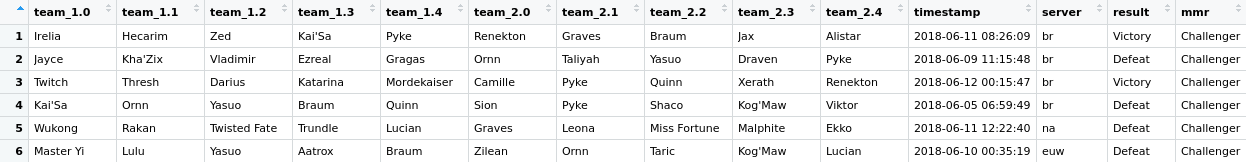
\includegraphics[width=15cm]{imagens/data_before}
\caption{\label{fig:dataantes}Conjunto de dados coletados}
\end{figure}

\begin{figure}[ht]
\centering
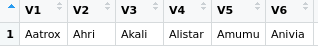
\includegraphics{imagens/champ_data}
\caption{\label{fig:champantes}Conjunto de dados dos personagens}
\end{figure}

A leitura dos dados ocorreu conforme o Código~\ref{cod:readinicio}. A variável \texttt{matches} corresponde ao conjunto de dados obtidos a partir da leitura do arquivo \texttt{patch811.csv} com a função \texttt{read.csv}. Para a leitura da lista de personagens foi executado a função \texttt{read.table}, pois os dados estavam dispostos no arquivo \texttt{champions.txt} separados por vírgula e em seguida foram armazenados na variável \texttt{champions}.

\begin{lstlisting}[language=R, caption={Leitura da 
base de dados original},label={cod:readinicio}]
# arquivo com os dados das partidas e carregado
matches <- read.csv('patch811.csv', stringsAsFactors = F)
# arquivo com a lista de personagens e carregado
champions <- read.table("champions.txt", sep=",")
\end{lstlisting}

\subsection{Formatação e Limpeza}
\label{sec:limpeza}

Após o carregamento dos dados, percebemos que seria importante a junção dos personagens de cada time em uma única coluna. Isto é, para o time 1, haveria uma coluna com os cinco personagens escolhidos, por sua vez, o time 2 também teria essa mesma representação em uma outra coluna. Se mantivéssemos o formato original, a análise seria mais complexa o que causaria dificuldades na elaboração de estatísticas.  

Sendo assim, concatenamos as variáveis que apresentam o nome dos personagens de cada time. Para tal etapa foi utilizada a função \texttt{unite} com o separador “\_”, como ilustrado no Código~\ref{cod:readdata}. Essa etapa foi realizada visando a simplificação das operações que podem ser realizadas usando as operações entre \textit{strings} contidas no R, assim criamos as colunas \texttt{team1} e \texttt{team2} (linhas 1-5 e 7-11, respectivamente). O segundo tratamento efetuado é a mudança do valor na variável \texttt{result}, que poderia ser \texttt{Victory} ou \texttt{Defeat}, para um valor booleano como \textit{True} ou \textit{False} (linhas 14 a 17). Essa operação simplifica qualquer outra operação futura pois esse valor poder ser facilmente convertido para inteiro e assim efetuar operações de soma ou média que serão utilizadas no projeto. Durante a leitura dos dados foi utilizada a função \texttt{read.csv} com todos os parâmetros padrões do R e o adiciona de \texttt{stringsAsFactors} como falso, visto no Código~\ref{cod:readinicio}. A Figura \ref{fig:data_clean} mostra o resultado obtido após a limpeza dos dados, as colunas exibidas são: \texttt{team1}, \texttt{team2}, \texttt{server}, \texttt{result} e \texttt{mmr}.

\begin{lstlisting}[language=R, caption={Leitura da base de dados},label={cod:readdata}]
# Concatena os valores das variaveis team1.x
matches <- matches %>%
    unite(col = "team1",
          1,2,3,4,5,
          sep = "_")
        
# Concatena os valores das variaveis team2.x
matches <- matches %>%
    unite(col = "team2",
          2,3,4,5,6,
          sep = "_")
          
# Substitui as strings por booleanos        
matches$result[matches$result=='Victory'] <- T
matches$result[matches$result=='Defeat'] <- F
# Converte para tipo 'logical'
matches$result <- as.logical(matches$result)
\end{lstlisting}


\begin{figure}[ht]
\centering
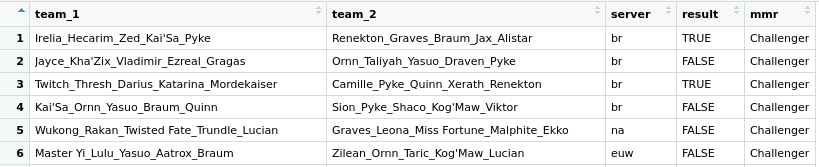
\includegraphics[width=15cm]{imagens/clean_data2}
\caption{\label{fig:data_clean}Dados após a limpeza}
\end{figure}

O outro conjunto de dados com a lista de personagens também precisa ser organizado em um formato mais amigável. O Código~\ref{cod:champlimpo} mostra a operação que foi realizada na variável \texttt{champions}. Aplicamos a função \texttt{gather} para transformar as colunas em linhas, para que assim tivéssemos apenas uma variável contendo a lista de personagens. Em seguida pegamos apenas os valores, transformando \texttt{champions} em uma lista com 143 elementos, como mostrado na Figura \ref{fig:names}. Portanto, obtemos todos os nomes possíveis para a composição de ambos os times. 

\begin{lstlisting}[language=R, caption={Organizando dados com os nomes dos personagens},label={cod:champlimpo}]
# Transforma as colunas em linhas
champions <- gather(champions, "champ")
# Obtem os valores da coluna e transforma em lista
champions <- champions$value
\end{lstlisting}


\begin{figure}
\centering
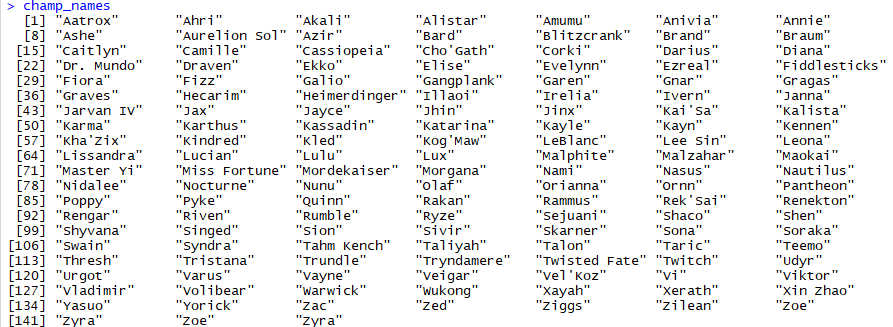
\includegraphics[width=15cm]{imagens/champ_names}
\caption{\label{fig:names}Nome dos personagens do jogo}
\end{figure}

Com os dados organizados e limpos, agora é possível analisar o conjunto de dados para propor melhores estatísticas com a finalidade de auxiliar no processo de escolha personagens em uma partida de LoL.

\section{Análise Exploratória}


Dado o conjunto de dados é possível extrair informações que antes não estava tão evidentes, informação como a taxa de vitória de uma personagem, podendo ser obtida de forma global (todas as regiões) ou local, e a popularidade de um personagem.

A taxa de vitória de um personagem pode ser algo associado ao \textit{patch} atual ou a popularidade dele, normalmente quando são feitos pequenos ajustes no jogo ou balanceamentos alguns dos personagens podem ganhar um pico de poder se comparado a sua versão antiga. Ou fator que pode influenciar nessa medida é o nível de dificuldade atrelado ao aprendizado com o uso de um certo personagem, certos personagens oferecem mecânicas mais simples e outros mais complexas. Quando um jogador mais experiente, geralmente nos ligas mais altas do jogo, ele possui certa facilidade com as mecânicas do jogo e esse fator quando aplicado em um personagem que está em seu pico de poder a taxa de vitória aumenta consideravelmente. 

No jogo a equipe SKT T1 da Coreia do Sul já foi considerada a melhor do mundo, nessa região o nível dos jogadores do competitivo é realmente alto se comparado com outras regiões. O jogador Faker (Lee Sang-hyeok), que joga na rota do meio, já foi considerado por muitos anos o melhor jogador em sua posição. Esse jogador tem um alto nível e quando em uma de suas partidas, seja em competições ou em partidas solo, e quando mostra um bom desempenho com algum personagem do jogo outros jogadores do mundo tentam “copiar” seu estilo de jogo, que se mostrou extremamente eficaz, e assim surgem os METAS.

\subsection{Taxa de Vitória}

A Figura~\ref{fig:win_rate} mostra dois gráficos: a direita com as melhores taxas de vitórias; a esquerda com as piores taxas de vitórias. Os valores do gráficos foram gerados usando o comando \texttt{head} para os melhores e \texttt{tail} para os piores. As barras indicam a taxa de vitória e a legenda mostra quais os seus valores utilizando as cores como referência. Com os dados apresentados nessa figura é possível observar que os personagens Quinn, Pantheon, Poppy, Cassiopeia e Kog’Maw obtiveram os melhores \textit{rates}, de forma global, todos acima de 50\%. Enquanto, Jinx, Amumu, Volibear, Tristana, Xerath e Elise apresentam os piores resultados, estes abaixo de 50\%. 

\begin{figure}[ht]
\centering
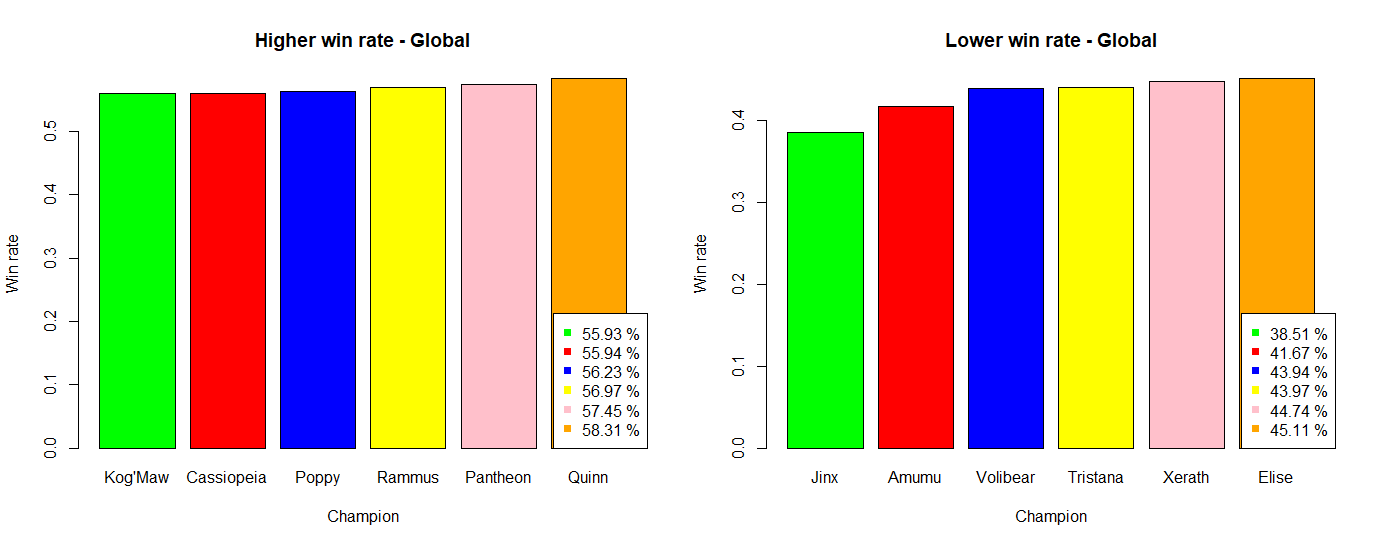
\includegraphics[width=1\columnwidth]{imagens/Rplot}
\caption{\label{fig:win_rate}Taxa de vitórias global}
\end{figure}

Os dados mostram que se um jogador for iniciar uma partida ou tentar melhorar com um novo personagem seria interessante observar jogos de um jogador mais experiente, facilmente encontrados em plataformas de \textit{streamming} como Youtube\footnote{https://www.youtube.com/} ou Twitch.tv\footnote{https://www.twitch.tv/}, e depois que entender a mecânica desse personagem inicia seus treinos. Usando uma estratégia assim o jogador pode atingir maiores taxa de vitória e usar o META e as estatísticas a seu favor.

\begin{lstlisting}[language=R, caption={Calculo da taxa de vitória},label={cod:win_rate}]

win_rate_final<-matrix(1:2*length(champ_names),length(champ_names),2)
for (x in 1:tamanho){
  champ_posicao<-which(grepl(champ_names[x],dados$team_1)) # Busca o time 1 que um persangem participou
  champ_posicao2<-which(grepl(champ_names[x],dados$team_2)) # Busca o time 2 que um persangem participou
  win_rate<-dados$result[champ_posicao] # Obtem o resultado do time 1
  win_temp<-!dados$result[champ_posicao2] # Obtem o resultado do time 2 (invertido)
  win_rate<-c(win_rate,win_temp) # Concatena os valores
  valor<-mean(win_rate) # Calcula a taxa de vitoria
  print(paste('Champion ', champ_names[x], ' possuiu uma win rate de ', valor, '!')) # Exibe o valor do resultado como o nome do personagem
  win_rate_final[x,1]<-valor # Salva o valor na matriz
  win_rate_final[x,2]<-champ_names[x] # Adiciona o nome do personagem na matriz
}

\end{lstlisting}

O código \ref{cod:win_rate} mostra como é efetuado o cálculo para a taxa de vitória, é feito uma busca para obter quais os times o personagem participou, depois é obtido o resultado da partida e por fim é utilizada a função \texttt{mean} para calcular o resultado final.

\begin{lstlisting}[language=R, caption={Código para gerar os gráfico dos dados},label={cod:win_rate_code}]
par(mfrow=c(1,2))
barplot(tail(data_champion$rate), 
        names.arg=tail(data_champion$names), 
        main="Higher win rate - Global",
        ylim=c(0,max(tail(data_champion$rate))),
        xlab="Champion",
        ylab="Win rate",
        col=colors)

legend("bottomright", legend = paste(round(tail(data_champion$rate), digits = 4)*100, '%'),
       col =colors, pch = 15)

barplot(head(data_champion$rate), 
        names.arg=head(data_champion$names), 
        main="Lower win rate - Global",
        ylim=c(0,max(head(data_champion$rate))),
        xlab="Champion",
        ylab="Win rate",
        col=colors)
legend("bottomright", legend = paste(round(head(data_champion$rate), digits = 4)*100, '%'),
       col =colors, pch = 15)

\end{lstlisting}


Código \ref{cod:win_rate_code} mostra como os gráficos foram gerados, como a quantidade de dados é grande foi optado o uso apenas do dados provenientes da função \texttt{head} e \texttt{tail}. Na parte inferior de cada barra é encontrado o nome do personagem e na legenda da imagem é apresentada o valor em percentual da respectiva taxa de vitória do personagem.
\subsection{Personagens Mais Populares}

No jogo como sabemos existem diferentes personagens com diferentes habilidades e dificuldades. Cabe ao jogador decidir durante uma partida qual personagem ele deseja. Essa escolha pode ter relação com o momento que o jogo se encontra, como exemplo, personagens ficaram mais fortes no \textit{patch} atual, novas mecânicas, ou até mesmo pelo fato de um personagem ter sido lançado recentemente. Diante disso, propomos um estilo de gráfico que representa os personagens mais e menos populares do jogo, isto é, quais personagens são mais e menos jogados.

A Figura~\ref{fig:popular} ilustra bem essa proposta. Diante dos gráficos é possível ter uma ideia dos personagens do momento. O gráfico da esquerda representa os personagens (\textit{champions}) mais escolhidos, nele listamos os 6 mais escolhidos dentre todas as regiões. Interpretando esses dados, podemos afirmar que nesse \textit{patch}, o personagem mais jogado é Lucian, com mais de 5000 partidas de um total de mais de 12 mil na base dados. Seguido pelos personagens Ezreal, Yasuo, Camile, Graves e Kai'sa. Isso pode representar que esses personagens estão fortes no META. Já o gráfico da direita mostra os personagens menos jogados, o que pode indicar que estes estão fracos em relação aos demais ou até mesmo o nível de dificuldade elevado durante uma partida. No gráfico o personagem menos jogado é Amumu com aproximadamente 60 partidas, seguido por Shyvana, Azir, Nasus, Volibear e Yorick.

\begin{figure}[ht]
\centering
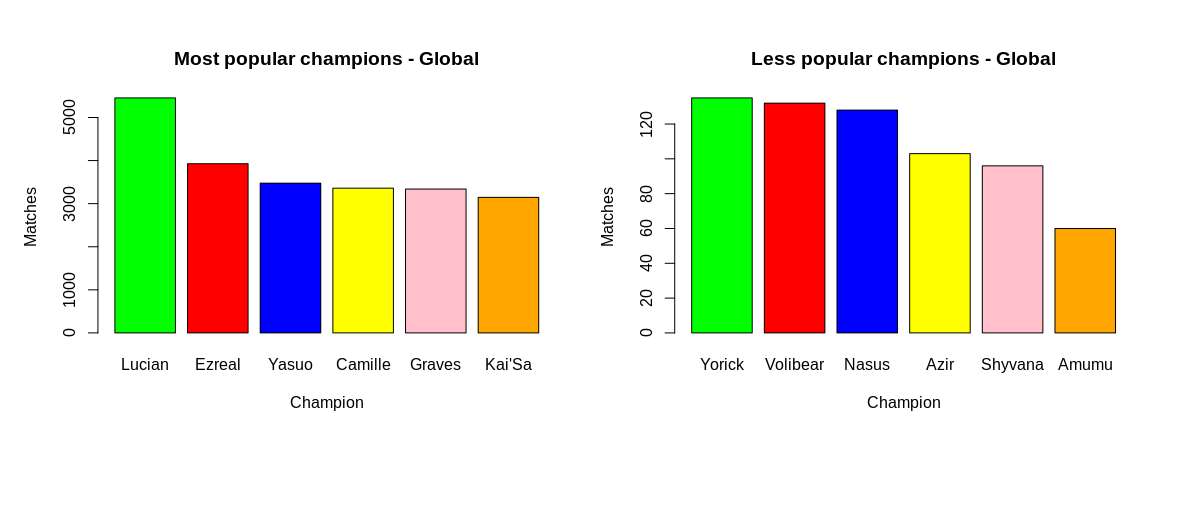
\includegraphics[width=1\columnwidth]{imagens/less_most_popular}
\caption{\label{fig:popular}Personagens mais e menos populares}
\end{figure}

Outro gráfico está ilustrado na Figura~\ref{fig:popular2}. Esse gráfico representa os campeões mais jogados por região, diferente do anterior que mostra a estatística global. Nele podemos notar que o campeão mais jogado é Lucian é o mais jogado em mais de uma região (\texttt{euw, na, br, las, eune}), o que confirma sua popularidade global em relação a Figura~\ref{fig:popular}. Além disso temos outros personagens: Zoe, Yasuo, Pyke e Taliah. Podemos notar que o personagem Yasuo em comparação com o resultado global é um dos mais jogador no servidor \texttt{br}, mas que no resultado geral é um dos menos jogados. Isso pode significar, que nessa região específica existam jogadores mais habilidosos com determinados campeões. Portanto, o cliente desses dados poderá usar um determinado personagem dependendo da região na qual o jogador está inserido.

\begin{figure}[ht]
\centering
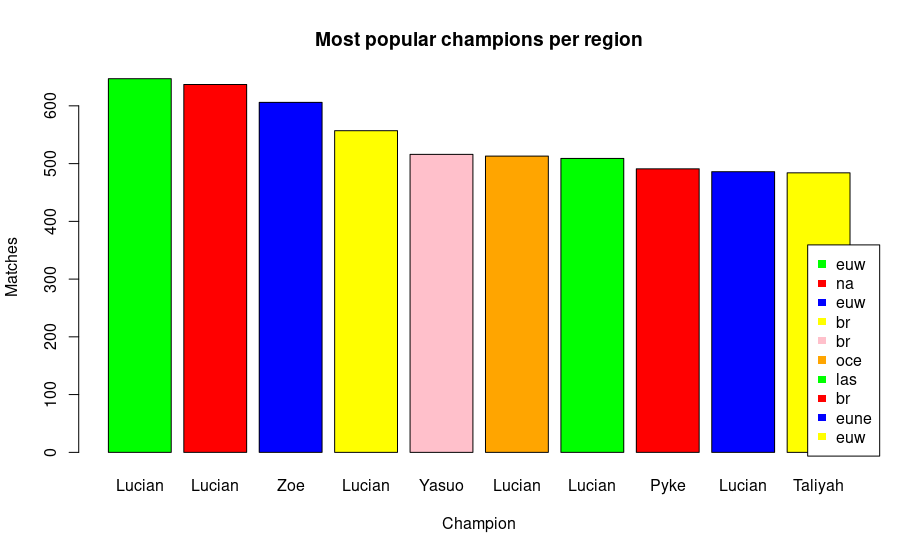
\includegraphics[width=0.7\columnwidth]{imagens/region}
\caption{\label{fig:popular2}Personagens mais populares por região (\textit{server})}
\end{figure}

Para gerar esses gráficos foi preciso um trabalho em cima da base de dados já organizada. O Código~\ref{cod:mostpop} mostra que para cada iteração ocorre sobre a lista de personagens (linhas 5 a 23), onde é obtido as posições onde há ocorrências do personagem \texttt{x} na base de dados \texttt{matches} através da função \texttt{grepl} aplicada à \texttt{which}. Isso ocorre para o time 1 e 2. Em seguida juntamos as bases \texttt{champ\_data\_team1} e \texttt{champ\_data\_team2} em um único conjunto de dados (\texttt{champ\_data}, linha 12) usando o comando \texttt{rbind}. Para agruparmos por região, aplicamos a função group\_by no conjunto de dados \texttt{champ\_data} na variável \texttt{server} (regiões). Em seguida é gerado um \textit{dataframe} com o cálculo da quantidade de partidas em cada região (linhas 16 a 22). O conjunto de dados \texttt{champ\_popularity} segue o padrão da Tabela~\ref{table:popregion}, onde para cada personagem há a quantidade de partidas (\textit{popularity}) em cada região (\textit{server}). Para gerar um conjunto dados com os personagens mais populares globalmente, utilizamos \texttt{group\_by} para agrupar os campeões (\texttt{champ}), em seguida é aplicado no \texttt{summarise} para gerar a quantidade (\texttt{count = sum(popularity.value)}) e ordenamos os dados com \texttt{arrange}. Para gerar os mais populares por região é similar, a diferença está no filtro aplicado ao \texttt{server} para ignorar elementos da região \texttt{www} (que representa um servidor de testes), e no agrupamento dos dados, pois utilizamos as variáveis \texttt{champ} e \texttt{populariy.server} (agrupando por personagem e servidor), assim aplicamos \texttt{summarise} para calcular o total (linhas 32 a 35).

\begin{lstlisting}[language=R, caption={Gerando novos dados a partir de um conjunto maior},label={cod:mostpop}]
# champiom's win rate by region
rate_by_region <- c()
regions <- unique(dados$server)
tamanho = length(champions)
for (x in 1:tamanho){
  champ_pos_team1 <- which(grepl(champions[x],matches$team1))
  champ_pos_team2 <- which(grepl(champions[x],matches$team2))
  champ_data_team1 <- matches[champ_pos_team1, ]
  champ_data_team2 <- matches[champ_pos_team2, ]
  champ_data_team2$result <- !champ_data_team2$result
  
  champ_data <- rbind(champ_data_team1, champ_data_team2)
  
  champ_popularity <- c()
  
  for(y in 1:length(regions)){
    champ_popularity[y] <- sum(champ_data$server == regions[y])
  }

  champ_popularity <- data.frame(server = regions, value = champ_popularity)
  
  rate_by_region <- rbind(rate_by_region, data.frame(champ=champions[x], champ_rate_by_region, popularity = champ_popularity))
}

# gera os personagens mais populares global
most_popular <- rate_by_region %>%
  group_by(champ) %>% # agrupa por personagem
  summarise(count = sum(popularity.value)) %>% # calcula a popularidade
  arrange(desc(count)) # ordena pela quantidade de partidas

# gera os personagens mais populares por regiao
most_popular_by_region <- rate_by_region %>%
  filter(popularity.server != "www")  %>%  # filtra o dado ignorando o servidor www
  group_by(champ, popularity.server) %>% # agrupa por personagem e regiao
  summarise(count = sum(popularity.value)) %>% # calcula a popularidade
  arrange(desc(count))
\end{lstlisting}

\begin{table}[ht]
\centering
\caption{Exemplo de dado gerado com popularidade}
\begin{tabular}{|l|l|l|}
\hline
\multicolumn{3}{|c|}{Aatrox} \\ \hline
 & server & popularity \\ \hline
1 & br & 59 \\ \hline
2 & na & 84 \\ \hline
3 & euw & 80 \\ \hline
4 & lan & 72 \\ \hline
5 & jp & 64 \\ \hline
6 & tr & 23 \\ \hline
\end{tabular}
\label{table:popregion}
\end{table}

Para gerar os gráficos apresentados na Figura~\ref{fig:popular} aplicamos o comando \texttt{barplot} pegando os seis personagens mais populares (\texttt{head(most\_popular\$champ)}) e os menos populares (\texttt{tail(most\_popular\$champ)}). Para o gráfico da Figura~\ref{fig:popular2} obtivemos os dez primeiros elemento do conjunto de dados. Aplicamos legendas e outros elementos visuais em todos eles, como está exposto no código. 

\begin{lstlisting}[language=R, caption={Gerando gráficos para mostrar visualmente a popularidade dos personagens},label={cod:mostpop}]
# coloca os graficos um ao lado do outro
par(mfrow=c(1,2))
# gera o grafico 1
barplot(head(most_popular$count), 
        names.arg=head(most_popular$champ), 
        main="Most popular champions - Global",
        xlab="Champion",
        ylab="Matches",
        col=colors)
legend("bottomright", legend = head(most_popular$champ),
       col =colors, pch = 15)
# gera o grafico 2
barplot(tail(most_popular$count), 
        names.arg=tail(most_popular$champ), 
        main="Less popular champions - Global",
        xlab="Champion",
        ylab="Matches",
        col=colors)
legend("bottomright", legend = tail(most_popular$champ),
       col =colors, pch = 15)
# gera o grafico dos personagens populares por regiao
barplot(most_popular_by_region$count[1:10], 
        names.arg=most_popular_by_region$champ[1:10], 
        main="Most popular champions per region",
        xlab="Champion",
        ylab="Matches",
        col=colors)
legend("bottomright", legend = most_popular_by_region$popularity.server[1:10],
       col =colors, pch = 15)
\end{lstlisting}



\subsection{Utilizando o KNN para previsão}

Já que os dados apresentam um conjunto de combinações de times e o resultado da partida é possível aplicar algoritmos como KNN (\textit{K nearest neighboors}) \cite{fukunaga1975branch}. Sua ideia principal é a possibilidade de estimar uma classe de um novo dado baseado no conjunto de vizinhos obtidos a partir de uma análise na base de dados. Para se estimar qual o nível de similaridade com um determinando elemento é utilizada uma função. Como os dados da base são apenas nomes dos personagens o cálculo é realizado utilizando quantos \textit{matches}, \texttt{str\_count} que conta a quantidade de ocorrências de \texttt{string} e um vetor , foram obtidos entre um time e toda a base dados. O resultado da partida, que pode ser vitória ou derrota, será obtido como a classe que foi associada a maioria dos vizinhos desse objeto avaliado. 

\begin{lstlisting}[language=R, caption={Código para calcular a similaridade de um elemento com a base de dados},label={cod:knn}]
df_knn<-data.frame(dist_team=rep(0,tamanho_base*2), classe = rep(0, tamanho_base*2))
for (x in 1:tamanho_base){
  df_knn$dist_team[x]<-sum(str_count(matches$team1[x], team)) # Utiliza sim para contar a quantidade de matchs
  df_knn$classe[x]<-matches$result[x] # Salva o resultado
  df_knn$dist_team[x+tamanho_base]<-sum(str_count(matches$team2[x], team)) # faz a contagem para o time 2
  df_knn$classe[x+tamanho_base]<-!matches$result[x] # inverte o resultado
}
df_knn<-df_knn[order(df_knn$dist_team, decreasing=TRUE),] # Ordena o vetor para obter os mais proximos

df_final<-df_knn[1:k,] # Obtem os k elementos mais proximos

if(length(df_final$classe[df_final$classe == 1]) > length(df_final$classe[df_final$classe == 0])){
  print("O time tem mais chances de vencer!")
}else if (length(df_final$classe[df_final$classe == 1]) < length(df_final$classe[df_final$classe == 0])){
  print("O time tem mais chances de perder!")
}else{
  print("O time tem as mesmas chances de vitoria e derrota!")
}
\end{lstlisting}


O código \ref{cod:knn} mostra como foi a implementação, a base de dados utiliza o mesmo pré-processamento utilizado para calcular as taxas de vitória, depois é calculada a distância para cada elemento utilizando a função  \texttt{str\_count} do pacote \texttt{stringr} que fornece a quantidade de \texttt{matches} (partidas). Como a base de dados, tanto do time 1 como do time 2, foi unida como uma única \texttt{string} que constitui o time inteiro, a função usada pode obter a quantidade de elementos que estão contidos no vetor, novo time avaliado, que se deseja comparar. Posteriormente é a verificação que tem como resultado se o time tem mais chances de vitória ou derreto e no caso para um k com valores pares a chance pode ser igual.
Utilizando o time com os personagens Graves, Ornn, Annie, Gragas, Alistar com o valor de $k=3$, o resultado obtido é "O time tem mais chances de perder!" os 5 elementos com maior proximidade apresentam uma quantidade de \texttt{matchs} sendo 3, que indica que 3 elementos desse tipo são similares a outros 3 elementos que constituem os times da base de dados. 
\section{Conclusões}

Neste trabalho aplicamos diferentes estatísticas em uma base de dados de partidas do jogo \textit{League of Legends}. A base de dados apresenta milhares de partidas que para o usuário não é possível entender e identificar \textit{insights}. Aplicamos técnicas e abordagens para tratar esses dados para que assim seja possível o usuário ver resultado de uma forma legível e de fácil interpretação.

Como a base de dados apresentavam informações sobre as partidas dos times e os respectivos personagens dos times para regiões específicas, propomos algumas estatísticas relacionadas aos próprios personagens. No caso, propomos estatísticas dos campeões com maiores taxas de vitória, os campeões mais populares e com isso pudemos prever possíveis resultados lavando em consideração um time fornecido pelo usuário, através do algoritmo k-NN. Portanto, gerando um indicativo por meio gráficos auxiliadores e informações em texto para quem está consultado essas informações antes de montar um time.

Um das limitações dessa proposta, é que os dados não são atualizados em tempo real, o que pode implicar em dados que não reflete à realidade, visto que o jogo está constantemente sofrendo atualizações e novas funcionalidades são disponibilizadas a cada \textit{patch}. Por isso seria importante, uma metodologia que utilizasse dados sempre atualizados e que levasse em consideração novas características do jogo, até mesmo com testes de hipóteses e outros meios estatísticos.

\renewcommand{\refname}{Referências}
\bibliographystyle{alpha}
\bibliography{sample}

\end{document}